\begin{pastexam}[label={px:ncu-113-dsa-01}]{中央資工所 113 學年度 第 1 題}
（複選；每題 5 分，全部答對才給分，答錯倒扣一分）

\begin{center}
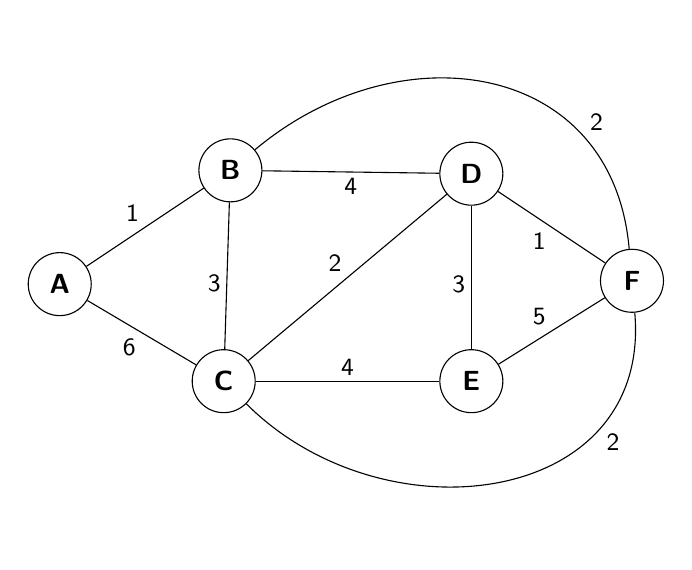
\begin{tikzpicture}[x=0.85cm,y=0.85cm,
  v/.style={circle,draw,minimum size=8mm,inner sep=0pt,font=\sffamily\bfseries},lab/.style={font=\sffamily\small,inner sep=2pt}]
\node[v] (A) at (1.2,-3.65) {A}; \node[v] (B) at (3.75,-1.95) {B}; \node[v] (C) at (3.65,-5.1) {C};
\node[v] (D) at (7.35,-2.0) {D}; \node[v] (E) at (7.35,-5.1) {E}; \node[v] (F) at (9.75,-3.6) {F};
\draw (A) -- node[lab,above left] {1} (B);
\draw (A) -- node[lab,below left] {6} (C);
\draw (B) -- node[lab,left,pos=0.55] {3} (C);
\draw (B) -- node[lab,below] {4} (D);
\draw (C) -- node[lab,above left] {2} (D);
\draw (C) -- node[lab,above] {4} (E);
\draw (D) -- node[lab,left,pos=0.55] {3} (E);
\draw (D) -- node[lab,below left] {1} (F);
\draw (E) -- node[lab,above left] {5} (F);
\draw (B) to[out=40,in=95,looseness=1.25] node[lab,above right,pos=0.75] {2} (F);
\draw (C) to[out=-45,in=-85,looseness=1.25] node[lab,below right,pos=0.75] {2} (F);
\end{tikzpicture}
\end{center}

Consider the graph above. Which of the following cannot be the edge selection sequence of Kruskal's
minimum spanning tree algorithm?
\begin{enumerate}[label=(\Alph*)]
\item (d, f) (a, b) (d, c) (b, f) (d, e)
\item (d, f) (a, b) (b, f) (d, e) (d, c)
\item (a, b) (d, f) (b, f) (f, c) (d, e)
\item (a, b) (d, f) (d, c) (f, c) (d, e)
\end{enumerate}
\end{pastexam}

\begin{pastsoln}
答案：(B)(D)。

圖上用大寫字母、選項用小寫，指的是同一組點。 邊依權重分組：
\begin{center}
\small
\begin{tabular}{cl}
\toprule
權重 & 邊 \\
\midrule
1 & A--B, D--F \\
2 & C--D, B--F, C--F \\
3 & B--C, D--E \\
4 & B--D, C--E \\
5, 6 & E--F, A--C \\
\bottomrule
\end{tabular}
\end{center}
Kruskal（資結書第~24.2~節）依權重由小到大看邊，兩端已經連通（加進去會成環）就跳過。 同權重的邊誰先
誰後可以任意，所以合法的選邊順序可能不只一種，但有兩個限制：選進來的邊權重不會變小；每一條選進來的邊
在當時不能和已選的邊成環。
\begin{itemize}
\item 權重 $1$：A--B、D--F 都選，順序任意。 之後的連通塊是 $\{A, B\}$、$\{D, F\}$、$\{C\}$、$\{E\}$。
\item 權重 $2$：C--D、B--F、C--F 三條。 B--F 連起 $\{A, B\}$ 和 $\{D, F\}$，一定會選。 C--D 和 C--F 都是把
C 接到 $\{D, F\}$，先看到的那條選進來，後看到的那條兩端已經連通（C--D--F 是一個三角形），跳過。
所以這一組選進兩條：B--F，加上 C--D 或 C--F 其中一條。 選完是 $\{A, B, C, D, F\}$、$\{E\}$。
\item 權重 $3$：B--C 兩端已連通，跳過；D--E 選進來，五條邊湊齊，結束。
\end{itemize}

逐項檢查：
\begin{itemize}
\item (A) (d, f) (a, b) (d, c) (b, f) (d, e)：權重 $1, 1, 2, 2, 3$，C--D 先於 C--F 被看到，合法。
\item (B) (d, f) (a, b) (b, f) (d, e) (d, c)：第四條選了權重 $3$ 的 D--E，第五條才選權重 $2$ 的 C--D。
Kruskal 看到 D--E 之前一定已經看過 C--D，那時 C 還沒和 D 連通，C--D 早就選進來了。 不可能，要選。
\item (C) (a, b) (d, f) (b, f) (f, c) (d, e)：這次是 C--F 先被看到，C--D 被跳過，合法。
\item (D) (a, b) (d, f) (d, c) (f, c) (d, e)：選了 C--D 之後 C、D、F 已經連通，C--F 會成環，不可能被選。
要選。
\end{itemize}
（(A)、(C) 的總權重都是 $1 + 1 + 2 + 2 + 3 = 9$。）
\end{pastsoln}
